\documentclass[xcolor={dvipsnames,table},aspectratio=169]{beamer}
\usepackage[utf8]{inputenc}
\usepackage[T1]{fontenc}
\usepackage[brazil]{babel}
\usepackage{graphics,amssymb,amsfonts,amsmath}
\usepackage{tikz}
\usepackage{enumerate,hyperref}
\usepackage{palatino}
\usepackage{ragged2e}
\usepackage{minted}
\usepackage{booktabs}
\usepackage{verbatim}
\usepackage[export]{adjustbox}
\usepackage{tikz}                   
\usepackage{xcolor}
\usepackage{textcomp} % para usar \textdegree
\usetikzlibrary{shadows}
\usetheme{AnnArbor}
\usecolortheme{orchid}
\usefonttheme[onlymath]{serif}

\newminted{java}{bgcolor=cyan!10}

\newcolumntype{C}[1]{>{\centering\let\newline\\\arraybackslash\hspace{0pt}}m{#1}}

\AtBeginSection[]{
  \begin{frame}
  \vfill
  \centering
  \begin{beamercolorbox}[sep=8pt,center,shadow=true,rounded=true]{title}
    \usebeamerfont{title}\insertsectionhead\par%
  \end{beamercolorbox}
  \vfill
  \end{frame}
}

\title[\sc{Laços}]{Laços}
\author[Roland Teodorowitsch]{Roland Teodorowitsch}
\institute[FPROG - EP - PUCRS]{Fundamentos de Programação - Escola Politécnica - PUCRS}
\date{24 de agosto de 2022}

\begin{document}
\justifying

%-------------------------------------------------------
\begin{frame}
	\titlepage
\end{frame}

%=======================================================
\section{Introdução}

%-------------------------------------------------------
\begin{frame}\frametitle{Objetivos}
\begin{itemize}
	\item Implementar laços com \texttt{while}, \texttt{for} e \texttt{do}
	\item Acompanhar a execução de um programa manualmente
	\item Familiarizar-se com os algoritmos comuns com laços
	\item Entender laços aninhados
	\item Implementar programas que leem e processam conjuntos de dados
\end{itemize}
\end{frame}

%-------------------------------------------------------
\begin{frame}\frametitle{Conteúdos}
\begin{itemize}
	\item O Laço \texttt{while}
	\item Resolução de Problemas: Teste de Mesa
	\item O Laço \texttt{for}
	\item O Laço \texttt{do}
	\item Sentinelas de Processamento
	\item Algoritmos Comuns com Laços
	\item Laços Aninhados
	\item Resolução de Problemas: \emph{Storyboards}
	\item Resumo
\end{itemize}
\end{frame}

%=======================================================
\section{O Laço \texttt{while}}

%-------------------------------------------------------
\begin{frame}[fragile]\frametitle{O Laço \texttt{while}}
\begin{itemize}
	\item Exemplos de aplicações com laços
	\begin{itemize}
		\item Cálculo de juros compostos
		\item Cálculo de um somatório
		\item Cálculo de um produtório
		\item Cálculo de média
		\item Simulações, programas orientados a eventos, etc.
	\end{itemize}
	\item Cálculo de juros compostos (Unidade 1)
\begin{verbatim}
Inicie com um valor de ano igual a zero e um total de $10.000
Repita o seguinte enquanto o total seja menor do que $20.000
     Adicione 1 ao valor do ano
     Multiplique o total por 1,05 (crescimento de 5%)
Informe o último valor atribuído ao ano como resposta
\end{verbatim}
\end{itemize}
\end{frame}

%-------------------------------------------------------
\begin{frame}[fragile]\frametitle{Planejando um Laço \texttt{while}}
\begin{columns}[T]
	\begin{column}{0.3\linewidth}
\begin{figure}[h]
	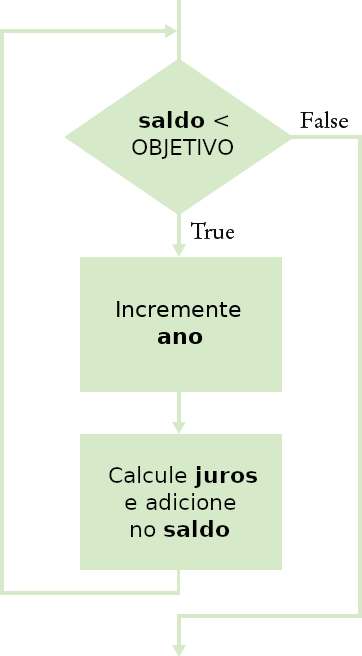
\includegraphics[height=0.65\paperheight,center]{pucrs-ep-fprog-unidade_04-lacos-laminas-fluxograma_laco.png}
\end{figure}
	\end{column}
	\begin{column}{0.7\linewidth}
		\begin{itemize}
		\item Um laço executa instruções repetidamente enquanto uma condição for verdadeira
\begin{javacode}
while (balance < TARGET) {
   year++;
   double interest = balance * RATE/100;
   balance = balance + interest;
}
\end{javacode}
		\end{itemize}
	\end{column}
\end{columns}
\end{frame}

%-------------------------------------------------------
\begin{frame}\frametitle{Sintaxe do Comando \texttt{while}}
\begin{figure}[h]
	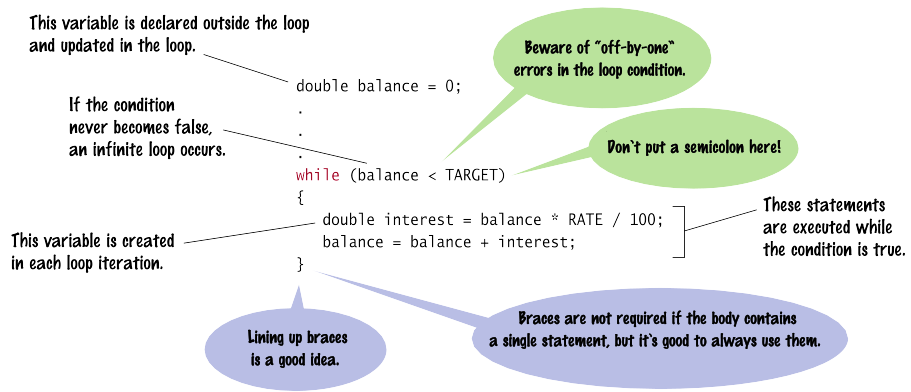
\includegraphics[height=0.65\paperheight,center]{pucrs-ep-fprog-unidade_04-lacos-laminas-sintaxe_while.png}
\end{figure}
\end{frame}

%-------------------------------------------------------
\begin{frame}[fragile]\frametitle{\texttt{DoubleInvestment.java} {\tiny (HORSTMANN, 2013, p. 143)}}
{\tiny
\begin{javacode}
/**
   This program computes the time required to double an investment.
*/
public class DoubleInvestment {
   public static void main(String[] args) {
      final double RATE = 5;
      final double INITIAL_BALANCE = 10000;
      final double TARGET = 2 * INITIAL_BALANCE;
      double balance = INITIAL_BALANCE;
      int year = 0;
      // Count the years required for the investment to double
      while (balance < TARGET) {
         year++;
         double interest = balance * RATE / 100;
         balance = balance + interest;
      }
      System.out.println("The investment doubled after "+ year + " years.");
   }
}
\end{javacode}
~\\
~\\
\textbf{Resultado da execução:}\\
\texttt{The investment doubled after 15 years.}
}
\end{frame}

%-------------------------------------------------------
\begin{frame}\frametitle{Execução do Laço (1)}
\begin{figure}[h]
	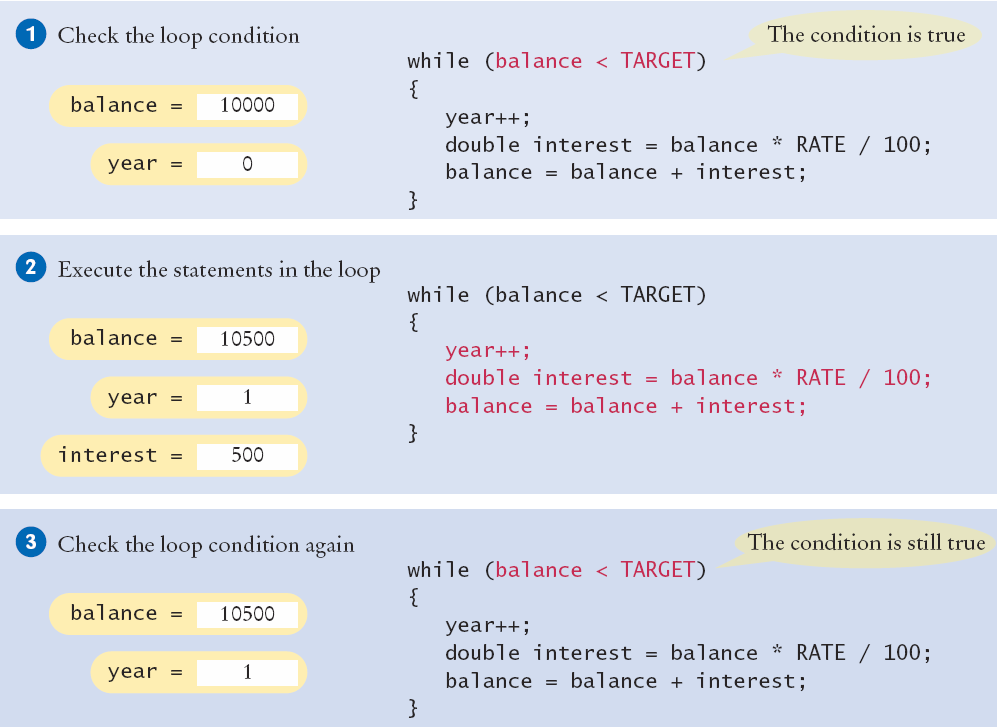
\includegraphics[height=0.70\paperheight,center]{pucrs-ep-fprog-unidade_04-lacos-laminas-execucao_do_laco_1.png}
\end{figure}
\end{frame}

%-------------------------------------------------------
\begin{frame}\frametitle{Execução do Laço (2)}
\begin{figure}[h]
	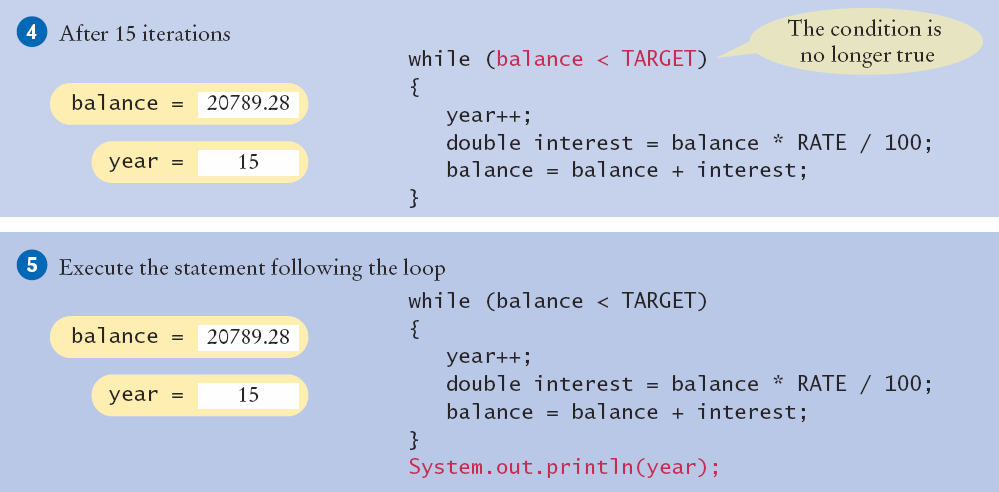
\includegraphics[height=0.50\paperheight,center]{pucrs-ep-fprog-unidade_04-lacos-laminas-execucao_do_laco_2.png}
\end{figure}
\end{frame}

%-------------------------------------------------------
\begin{frame}[fragile]\frametitle{Exemplos de Laços com \texttt{while} (1)}
{\scriptsize
\begin{center}
  \begin{tabular}{|p{6cm}|p{2cm}|p{5cm}|}
\hline
    \textbf{Laço} & \textbf{Saída} & \textbf{Explicação} \\
\hline
{\tiny
\begin{minted}{java}
i = 0; sum = 0;
while (sum < 10) {
   i++; sum = sum + i;
   System.out.println(i+" "+sum);
}
\end{minted}
}
&
{\tiny
\begin{verbatim}
1 1
2 3
3 6
4 10
\end{verbatim}
}
& Quando \texttt{sum} for igual a $10$, a condição do laço será falsa, e o laço se encerra.\\
\hline
{\tiny
\begin{minted}{java}
i = 0; sum = 0;
while (sum < 10) {
   i++; sum = sum - i;
   System.out.println(i+" "+sum);
}
\end{minted}
}
&
{\tiny
\begin{verbatim}
1 -1
2 -3
3 -6
4 -10
...
\end{verbatim}
}
& Como \texttt{sum} nunca atinge $10$, isto consiste em um ``laço infinito''.\\
\hline
{\tiny
\begin{minted}{java}
i = 0; sum = 0;
while (sum < 0) {
   i++; sum = sum - i;
   System.out.println(i+" "+sum);
}
\end{minted}
}
&
(Nenhuma saída)
& A condição \texttt{sum < 0} é falsa quando é testada pela primeira vez, e o laço nunca é executado.\\
\hline
  \end{tabular}
\end{center}
}
\end{frame}

%-------------------------------------------------------
\begin{frame}[fragile]\frametitle{Exemplos de Laços com \texttt{while} (2)}
{\scriptsize
\begin{center}
  \begin{tabular}{|p{6cm}|p{2cm}|p{5cm}|}
\hline
    \textbf{Laço} & \textbf{Saída} & \textbf{Explicação} \\
\hline
\begin{minted}{java}
i = 0; sum = 0;
while (sum >= 10) {
   i++; sum = sum + i;
   System.out.println(i+" "+sum);
}
\end{minted}
&
(Nenhuma saída)
& O programador provavelmente pensou: ``Pare quando a soma for pelo menos $10$''. Entretanto a condição do laço controla quando o laço é executado, e não quando ele se encerra.\\
\hline
\begin{minted}{java}
i = 0; sum = 0;
while (sum < 10) ; {
   i++; sum = sum + i;
   System.out.println(i+" "+sum);
}
\end{minted}
&
(Nenhuma saída e o programa nunca termina)
& Observe que o ponto-e-vírgula após o teste do laço faz com que o corpo do laço corresponda a um comando vazio. O programa executará para sempre pois \texttt{sum < 0} e este valor não será atualizado no corpo do laço (comando vazio).\\
\hline
  \end{tabular}
\end{center}
}
\end{frame}

%-------------------------------------------------------
\begin{frame}[fragile]\frametitle{Erros Comuns (1)}
Não pense: ``Já chegamos lá?''
\begin{itemize}
	\item O corpo do laço somente será executado se a condição de teste for verdadeira
	\item A lógica para ``Já chegamos lá?'' executaria o corpo do laço se o teste fosse falso
	\item Se \texttt{bal} deve crescer até que alcance \texttt{TARGET}, qual versão executará o corpo do laço?
\begin{columns}[T]
	\begin{column}{0.5\linewidth}
\begin{javacode}
while (bal < TARGET) {
   year++;
   interest = bal * RATE;
   bal = bal + interest;
}
\end{javacode}
	\end{column}
	\begin{column}{0.5\linewidth}
\begin{javacode}
while (bal >= TARGET) {
   year++;
   interest = bal * RATE;
   bal = bal + interest;
}
\end{javacode}
	\end{column}
\end{columns}
\end{itemize}
\end{frame}

%-------------------------------------------------------
\begin{frame}[fragile]\frametitle{Erros Comuns (2)}
Laços Infinitos
\begin{itemize}
	\item O corpo do laço será executado até que a condição de teste se torne falsa
	\item O que acontece se você se esquecer de atualizar a variável de teste?
	\begin{itemize}
		\item \texttt{bal} é a variável de teste (\texttt{TARGET} não é alterado)
		\item Seu programa ficará no laço para sempre! (ou até que você pare o programa)
	\end{itemize}
\begin{javacode}
while (bal < TARGET) {
   year++;
   interest = bal * RATE;
   // bal = bal + interest;
}
\end{javacode}
\end{itemize}
\end{frame}

%-------------------------------------------------------
\begin{frame}[fragile]\frametitle{Erros Comuns (3)}
Erros de Limite
\begin{itemize}
	\item Uma variável do tipo contadora é frequentemente usada na condição de teste
	\item A variável contadora pode iniciar em 0 ou 1 (programadores frequentemente iniciam contadores com 0)
	\item Se você quer contar 5 dedos, qual código deve ser usado?
\begin{columns}[T]
	\begin{column}{0.5\linewidth}
\begin{javacode}
// Inicia em 0, usa-se <
int finger = 0;
final int FINGERS = 5;
while (finger < FINGERS) {
   System.out.println(finger);
   finger++;
}
// 0,1,2,3,4
\end{javacode}
	\end{column}
	\begin{column}{0.5\linewidth}
\begin{javacode}
// Inicia em 1, usa-se <=
int finger = 1;
final int FINGERS = 5;
while (finger <= FINGERS) {
   System.out.println(finger);
   finger++;
}
// 1,2,3,4,5
\end{javacode}
	\end{column}
\end{columns}
\end{itemize}
\end{frame}

%-------------------------------------------------------
\begin{frame}\frametitle{Resumo do Laço \texttt{while}}
\begin{itemize}
	\item Laços com \texttt{while} são usados com grande frequência
	\item Inicialize as variáveis antes do teste
	\item A condição é testada ANTES do corpo do laço
	\begin{itemize}
		\item Isto é chamado pré-teste
		\item A condiçao frequentemene usa uma variável contadora
	\end{itemize}
	\item Algo dentro do corpo do laço deve alterar uma das variáveis usadas no teste
	\item Cuidado com laços infinitos!
\end{itemize}
\end{frame}

%-------------------------------------------------------
\begin{frame}\frametitle{Exercícios}
Faça laços em Java usando \texttt{while} para mostrar:
\begin{enumerate}
	\item Os números inteiros de 100 a 200
	\item Os números inteiros de -10 a -50
	\item Os números pares entre \texttt{a} e \texttt{b} (com \texttt{a} $\ge$ \texttt{b})
	\item As 10 primeiras potências de 2
	\item Os elementos de uma progressão aritmética de \texttt{n} elementos que inicia em \texttt{a} e tem razão \texttt{r}
	\item A soma dos elementos do item anterior
	\item Os elementos de uma progressão geométrica de \texttt{n} elementos que inicia em \texttt{a} e tem razão \texttt{r}
	\item A soma dos elementos do item anterior
\end{enumerate}
\end{frame}

%=======================================================
\section{Resolução de Problemas: Teste de Mesa}

%-------------------------------------------------------
\begin{frame}[fragile]\frametitle{Teste de Mesa}
Exemplo: Calcule a soma dos dígitos de um número (por exemplo, para 1729 o valor seria 1+7+2+9)
\begin{itemize}
	\item Faça colunas para as principais variáveis (\texttt{n}, \texttt{sum}, \texttt{digit})
	\item Acompanhe a execução e mantenha os valores das variáveis atualizados na tabela
\begin{javacode}
int n = 1729;
int sum = 0;
while (n > 0) {
   int digit = n % 10;
   sum = sum + digit;
   n = n / 10;
}
System.out.println(sum);
\end{javacode}
\end{itemize}
\end{frame}

%=======================================================
\section{Exercícios}

%-------------------------------------------------------
\begin{frame}\frametitle{Exercícios (1)}
Escreva laços \texttt{while} em Java, declarando todas as variáveis utilizadas, para:
\begin{enumerate}
	\item Mostrar os valores de 1 até 10.
	\item Mostrar os valores de 10 até 1, em ordem regressiva.
	\item Calcular a soma dos valores de 1 até 20.
	\item Calcular o fatorial de um número inteiro lido do terminal.
	\item Ler 20 pares de valores (\texttt{a} e \texttt{b}) escrevendo qual é o maior valor.
	\item Ler um número inteiro e escrever se ele é primo ou não.
\end{enumerate}
\end{frame}

%-------------------------------------------------------
\begin{frame}[fragile]\frametitle{Exercícios (2)}
Faça o teste de mesa para o trecho de programa em Java a seguir, mostrando todas as alterações de valores nas variáveis declaradas e todas as saídas de terminal, e considerando que os valores lidos do teclado serão respectivamente 2, 4, 3, 2, 0, 2.\\
{\scriptsize
\begin{javacode}
Scanner in = new Scanner(System.in);
int x, a, n, z;

x = in.nextInt();
n = in.nextInt();
while (x > 0) {
   a = 1;
   while (a <= n) {
      z=a*n;
      System.out.println(z);
      a = a + 1;
   }
   x = in.nextInt();
   n = in.nextInt();
}
\end{javacode}
}
\end{frame}

%=======================================================
\section{O Laço \texttt{for}}

%-------------------------------------------------------
\begin{frame}[fragile]\frametitle{O Laço \texttt{for}}
\begin{itemize}
    \item Em Java, tudo que é feito com \texttt{while} pode ser feito também com \texttt{for}
    \item Mas use laços \texttt{for} quando 
	\begin{itemize}
		\item Houver uma variável de indução com início, atualização e fim claramente identificáveis
		\item For interessante deixar o código mais conciso (controle do laço em uma única linha)
	\end{itemize}
	\item Por exemplo, para fazer o somatório dos números de 1 até 10 poderíamos fazer:
	
\begin{columns}[T]
	\begin{column}{0.5\linewidth}
{\scriptsize
\begin{javacode}
int soma = 0;
// versao com while
int i = 1;  // inicializacao
while (i <= 10)  { // teste
   soma = soma + i;
   i++; // atualizacao
}
\end{javacode}
}
	\end{column}
	\begin{column}{0.5\linewidth}
{\scriptsize
\begin{javacode}
int soma = 0;
// versao com for
for (int i = 1; i <= 10; i++) {
   soma = soma + i;
}
\end{javacode}
}
\end{column}
\end{columns}
\end{itemize}
\end{frame}

%-------------------------------------------------------
\begin{frame}[fragile]\frametitle{Sintaxe do Comando \texttt{for}}
\begin{javacode}
for ( inicializacao; condicao; atualizacao)
    corpo;
\end{javacode}
\begin{itemize}
    \item O comando \texttt{for} tem 4 partes:
    \begin{enumerate}
        \item Inicialização: é executada uma vez antes do laço iniciar
        \item Condição de permanênica: é verificada antes de cada iteração (deve ser verdadeira)
        \item Corpo do laço (bloco de comandos ou comando único): executado enquanto a condição for verdadeira
        \item Atualização: executada sempre depois do bloco de comandos e antes de se fazer um novo teste da condição
    \end{enumerate}
    \item Depois da inicialização, o laço \texttt{for} repetirá um ciclo formado por
    \begin{itemize}
        \item Teste da condição --- Execução do corpo do laço --- Atualização
    \end{itemize}
\end{itemize}
\end{frame}

%-------------------------------------------------------
\begin{frame}\frametitle{Execução de um laço \texttt{for}}
\begin{figure}[h]
	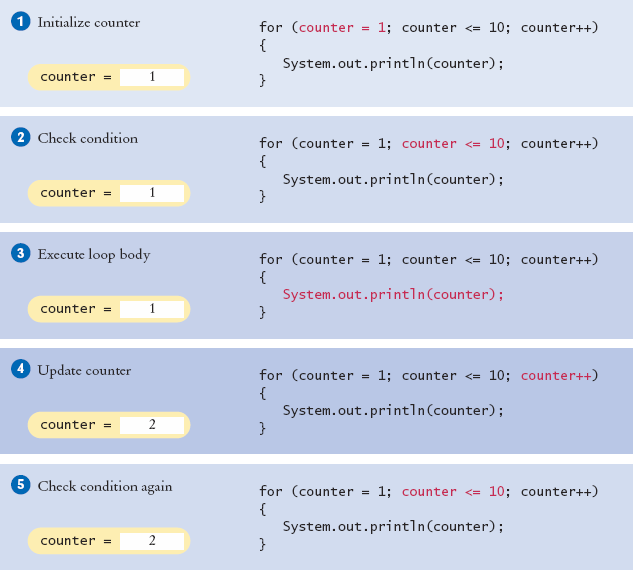
\includegraphics[height=0.70\paperheight,center]{pucrs-ep-fprog-unidade_04-lacos-laminas-execucao_do_laco_for.png}
\end{figure}
\end{frame}

%-------------------------------------------------------
\begin{frame}[fragile]\frametitle{Exemplos de Laços \texttt{for} (1)}
\begin{itemize}
\item Contar de 1 (inclusive) até 5 (inclusive) [5 iterações: 1 2 3 4 5]
{\scriptsize
\begin{javacode}
for (int i = 1; i<=5; i++) System.out.println(i);
for (int i = 1; i<6; i++) System.out.println(i);
\end{javacode}
}
\item Contar de 1 (inclusive) até 5 (exclusive) [4 iterações: 1 2 3 4]
{\scriptsize
\begin{javacode}
for (int i = 1; i<=4; i++) System.out.println(i);
for (int i = 1; i<5; i++) System.out.println(i);
\end{javacode}
}
\item Contar de 0 (inclusive) até 5 (inclusive) [6 iterações: 0 1 2 3 4 5]
{\scriptsize
\begin{javacode}
for (int i = 0; i<=5; i++) System.out.println(i);
for (int i = 0; i<6; i++) System.out.println(i);
\end{javacode}
}
\item Contar de 0 (inclusive) até 5 (exclusive) [5 iterações: 0 1 2 3 4]
{\scriptsize
\begin{javacode}
for (int i = 0; i<=4; i++) System.out.println(i);
for (int i = 0; i<5; i++) System.out.println(i);
\end{javacode}
}
\end{itemize}
\end{frame}

%-------------------------------------------------------
\begin{frame}[fragile]\frametitle{Exemplos de Laços \texttt{for} (2)}
\begin{itemize}
\item Contagem regressiva [6 iterações: 5 4 3 2 1 0]
{\scriptsize
\begin{javacode}
for (int i = 5; i>=0; i--) System.out.println(i);
\end{javacode}
}
\item Incremento igual a 2 [5 iterações: 0 2 4 6 8]
{\scriptsize
\begin{javacode}
for (int i = 0; i<9; i=i+2) System.out.println(i);
\end{javacode}
}
\item Razão geométrica igual a 2 [5 iterações: 1 2 4 8 16]
{\scriptsize
\begin{javacode}
for (int i = 1; i<=20; i=i*2) System.out.println(i);
\end{javacode}
}
\item Percorrer todas as letras de uma cadeia de caracteres [4 iterações: J A V A]
{\scriptsize
\begin{javacode}
String s = "JAVA";
for (int i = 0; i<s.length(); i++) System.out.println(s.charAt(i));
\end{javacode}
}
\end{itemize}
\end{frame}

%-------------------------------------------------------
\begin{frame}[fragile]\frametitle{Planejando um Laço \texttt{for}}
\begin{columns}[T]
	\begin{column}{0.3\linewidth}
\begin{figure}[h]
	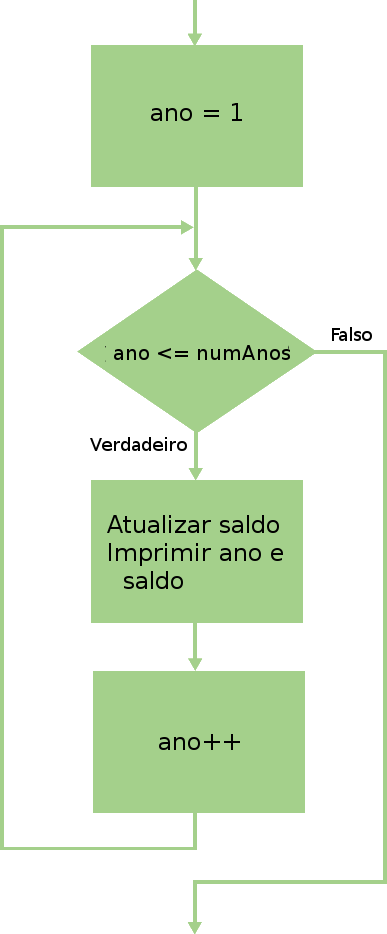
\includegraphics[height=0.70\paperheight,center]{pucrs-ep-fprog-unidade_04-lacos-laminas-fluxograma_laco_for.png}
\end{figure}
	\end{column}
	\begin{column}{0.7\linewidth}
	\begin{itemize}
        {\footnotesize
		\item Considerando um valor inicial investido de 10000, e uma taxa de juros anual de 5\%, escreva um programa que: leia o número total de anos de investimento (\texttt{numAnos}) e, para cada ano transcorrido, imprima o número do ano e o saldo total ao final desse ano.
		\item Por exemplo, para \texttt{numAnos} igual a 5, o programa deve imprimir:
		}
		\begin{itemize}
            {\scriptsize
			\item ano 1: 10500.00
			\item ano 2: 11025.00
			\item ano 3: 11576.25
			\item ano 4: 12155.06
			\item ano 5: 12762.82\\
			}
		\end{itemize}
	\end{itemize}
{\scriptsize
\begin{javacode}
for (int ano = 1; ano <= numAnos; ano++) {
   // Atualiza saldo
   // Imprime ano e saldo
}
\end{javacode}
}
	\end{column}
\end{columns}
\end{frame}

%-------------------------------------------------------
\begin{frame}[fragile]\frametitle{\texttt{Investimento.java}}
{\tiny
\begin{javacode}
import java.util.Scanner;

/**
   Este programa imprime uma tabela mostrando o crescimento anual de um investimento.
*/
public class Investimento {
   public static void main(String[] args) {
      final double TAXA = 5.0;
      final double SALDO_INICIAL = 10000;
      double saldo = SALDO_INICIAL;

      System.out.print("Quantos anos? ");
      Scanner in = new Scanner(System.in);
      int numAnos = in.nextInt();

      for (int ano = 1; ano <= numAnos; ano++) {
         double juros = saldo * TAXA / 100.0;
         saldo = saldo + juros;
         System.out.printf("ano %d: %.2f\n", ano, saldo);
      }
   }
}
\end{javacode}
}
\end{frame}

%-------------------------------------------------------
\begin{frame}[fragile]\frametitle{Cuidados a serem tomados}
\begin{itemize}
    \item Limite final do laço: inclusive ou exclusive?
    \item Variável de indução: crescente ou decrescente?
    \begin{itemize}
        \item Com valores crescentes usa-se $\le$ ou $<$
        \item Com valores decrescentes usa-se $\ge$ ou $>$
    \end{itemize}
    \item Condições erradas podem gerar \textbf{laços infinitos}:
{\scriptsize
\begin{javacode}
// 0 2 4 6 8 10 ...
for (int i=0; i!=9; i=i+2) System.out.println(i);

// 0 -1 -2 -3 -4 -5 ...
for (int i=0; i<10; --i) System.out.println(i);
\end{javacode}
}
	\item Evite atualizar o contador no corpo do laço \texttt{for}:
{\scriptsize
\begin{javacode}
for (int i=1; i<=100; i++) {
   if (i % 10 == 0)       // Pular valores divisiveis por 10
      i++;                // Estilo ruim para for...
   System.out.println(i);
}
\end{javacode}
}
\end{itemize}
\end{frame}

%-------------------------------------------------------
\begin{frame}[fragile]\frametitle{Escopo de Variáveis do Laço \texttt{for}}
\begin{itemize}
	\item Escopo é o ``tempo de vida'' de uma variável.
	\item Quando a variável \texttt{x} é declarada no comando \texttt{for}, ela existe apenas dentro do bloco do laço
\begin{javacode}
for ( int x = 1; x < 10; x = x + 1) {
   // comandos a serem executados dentro do laco
   // 'x' pode ser usado em qualquer lugar dentro deste bloco
}
if (x > 100)   // Erro! 'x' esta fora de escopo!
\end{javacode}
	\item Solução: declarar 'x' fora do laço
\begin{javacode}
int x;
for ( x = 1; x < 10; x = x + 1) {}
\end{javacode}
\end{itemize}
\end{frame}

%-------------------------------------------------------
\begin{frame}\frametitle{Resumo do Laço \texttt{for}}
\begin{itemize}
	\item Laços com \texttt{for} são muito usados
	\item Eles têm uma notação bastante concisa
	\begin{itemize}
		\item Inicialização ; Condição ; Atualização ; Corpo do laço
		\item A inicialização acontece uma única vez no início do laço
		\item A condição é testada todas as vezes ANTES (pré-teste) de executar o corpo do laço
		\item O incremento é realizado APÓS o corpo do laço
	\end{itemize}
	\item Use laços \texttt{for} seguindo o modelo padrão
	\item Adequado para contagens inteiras, processamento de \emph{strings}, vetores ou matrizes, etc.
\end{itemize}
\end{frame}

%=======================================================
\section{Exercícios sobre Laço \texttt{for}}

%-------------------------------------------------------
\begin{frame}\frametitle{Exercícios 1 e 2}
\begin{enumerate}
    \item Escreva laços \texttt{for} em Java, declarando todas as variáveis utilizadas, para:
    \begin{enumerate}[a.]
        \item Mostrar os valores de 1 até 10.
        \item Mostrar os valores de 10 até 1, em ordem regressiva.
        \item Calcular a soma dos valores de 1 até 20.
        \item Calcular o fatorial de um número inteiro lido do terminal.
        \item Ler 20 pares de valores (\texttt{a} e \texttt{b}) escrevendo qual é o maior valor.
        \item Ler um número inteiro e escrever se ele é primo ou não.
    \end{enumerate}
    \item Escreva um programa em Java para ler o número de alunos de uma turma e a seguir ler as notas destes alunos na prova da disciplina, determinando e imprimindo: a média da turma, a nota mais baixa e a nota mais alta.
\end{enumerate}
\end{frame}

%-------------------------------------------------------
\begin{frame}[fragile]\frametitle{Exercício 3}
\begin{enumerate}
    \setcounter{enumi}{2}
    \item Faça o teste de mesa para o trecho de programa em Java a seguir, mostrando todas as alterações de valores nas variáveis declaradas e todas as saídas de terminal, e considerando que os valores lidos do teclado serão respectivamente 4, 2, 2, 3, 2, 0.
{\scriptsize
\begin{javacode}
Scanner in = new Scanner(System.in);
int x, a, n, z;

n = in.nextInt();
for ( x = in.nextInt() ; x > 0 ; x = in.nextInt() ) {
   for ( a = 1 ; a <= n ; a = a + 1 ) {
      z=a*n;
      System.out.println(z);
   }
   n = in.nextInt();
}
\end{javacode}
}
\end{enumerate}
\end{frame}

%=======================================================
\section{O Laço \texttt{do}}

%-------------------------------------------------------
\begin{frame}[fragile]\frametitle{O Laço \texttt{do}}
\begin{columns}[T]
	\begin{column}{0.3\linewidth}
\begin{figure}[h]
	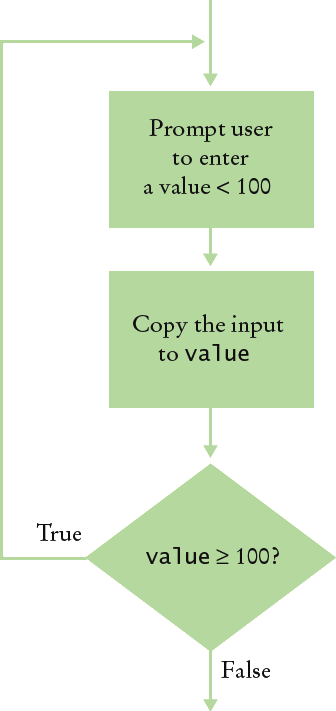
\includegraphics[height=0.65\paperheight,center]{pucrs-ep-fprog-unidade_04-lacos-laminas-fluxograma_laco_do.png}
\end{figure}
	\end{column}
	\begin{column}{0.7\linewidth}
\begin{itemize}
	\item Usa-se o laço \texttt{do} quando se deseja executar o corpo do laço pelo menos uma vez, testando a condição APÓS a primeira repetição do laço
\end{itemize}
\begin{javacode}
int i = 1;  // inicializacao
final int FINGERS = 5;
do {
   // comandos...
   i++; // atualizacao
}  while (i <= FINGERS);  // teste
\end{javacode}
	\end{column}
\end{columns}

\end{frame}

%-------------------------------------------------------
\begin{frame}[fragile]\frametitle{Exemplo de Laço \texttt{do}}
\begin{itemize}
	\item Validação da entrada de usuários
	\begin{itemize}
		\item Verificar se um valor lido está dentro do limite
		\item O usuário tem que fornecer alguma entrada antes para ser validada 
	\end{itemize}
\end{itemize}
\begin{javacode}
int valor;
do {
   System.out.println("Forneca um valor inteiro < 100: "); 
   valor = in.nextInt();
}  while (valor >= 100);  // Teste
\end{javacode}
\end{frame}

%-------------------------------------------------------
\begin{frame}\frametitle{Dica de Programação}
\begin{itemize}
	\item Fluxogramas para laços: evite código "spaghetti" (nunca faça uma seta apontar para dentro do corpo de um laço)
\end{itemize}
\begin{columns}[T]
	\begin{column}{0.5\linewidth}
\begin{center}
\texttt{while} e \texttt{for} testam antes
\begin{figure}[h]
	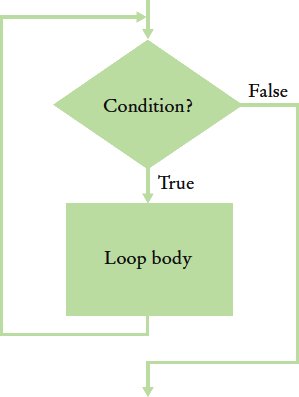
\includegraphics[height=0.4\paperheight,center]{pucrs-ep-fprog-unidade_04-lacos-laminas-fluxograma_teste_antes.png}
\end{figure}
\end{center}
	\end{column}
	\begin{column}{0.5\linewidth}
\begin{center}
\texttt{do} testa depois
\begin{figure}[h]
	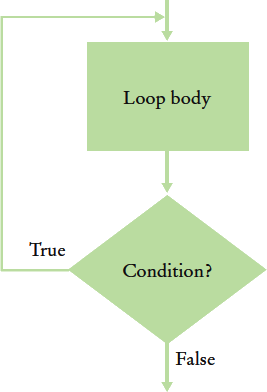
\includegraphics[height=0.4\paperheight,center]{pucrs-ep-fprog-unidade_04-lacos-laminas-fluxograma_teste_depois.png}
\end{figure}
\end{center}
	\end{column}
\end{columns}

\end{frame}

%-------------------------------------------------------
\begin{frame}\frametitle{Humor}
\begin{figure}[h]
	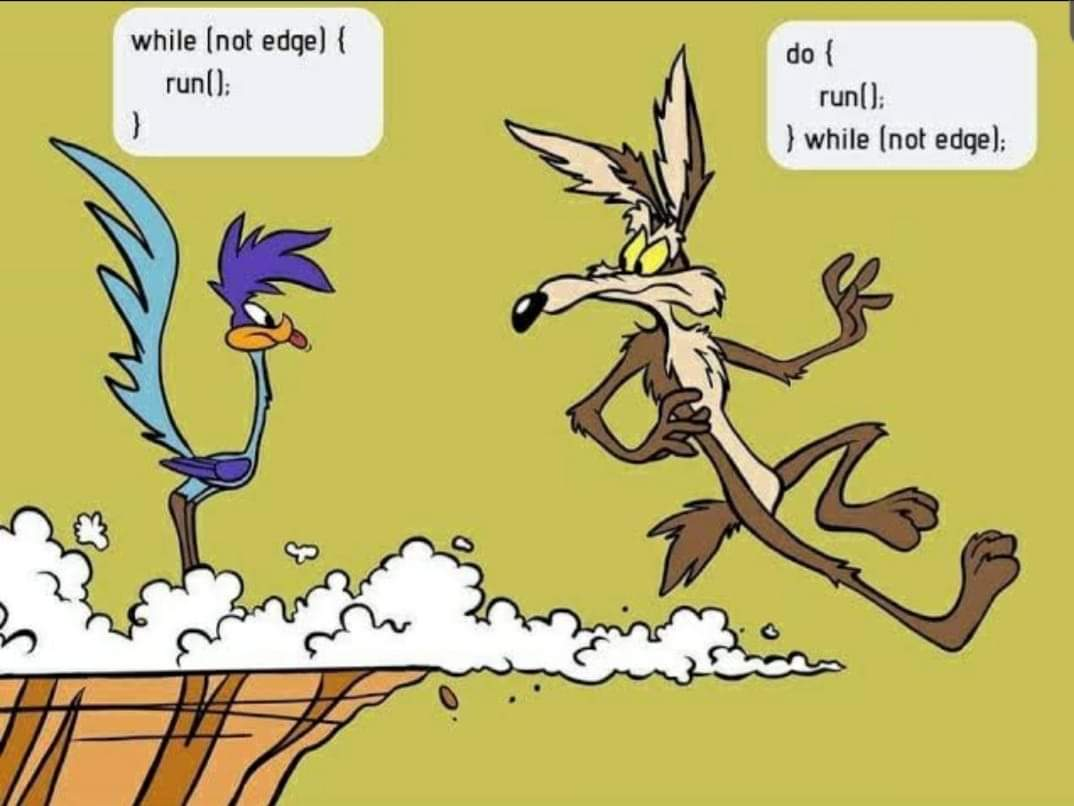
\includegraphics[height=0.7\paperheight,center]{pucrs-ep-fprog-unidade_04-lacos-laminas-while_vs_do_while.jpg}
\end{figure}
\end{frame}

%=======================================================
\section{Sentinelas de Processamento}

%-------------------------------------------------------
\begin{frame}[fragile]\frametitle{Sentinelas de Processamento}
\begin{itemize}
	\item Valores de sentinela indicam o final de um conjunto de dados, mas não fazem parte dos dados
	\item Podem ser usados em muitos casos
	\begin{itemize}
		\item Quando não se sabe quantos itens há em uma lista, usa-se um caracter ou valor especial para sinalizar que não há mais itens
		\item Para entradas de números positivos, é comum usar o valor -1:
\begin{javacode}
salary = in.nextDouble();
while (salary != -1) {
   sum = sum + salary;
   count++;
   salary = in.nextDouble();
}
\end{javacode}
	\end{itemize}
\end{itemize}
\end{frame}

%-------------------------------------------------------
\begin{frame}\frametitle{Calculando a Média de um Conjunto Indeterminado de Valores}
\begin{itemize}
	\item Declare e inicialize uma variável \texttt{sum} com 0
	\item Declare e inicialize uma variável \texttt{count} com 0
	\item Declare e inicialize uma variável \texttt{input} com 0
	\item Mostre uma mensagem solicitando que o usuário forneça os dados
	\item Fique no laço até que o valor de sentinela seja fornecido
	\begin{itemize}
		\item Leia um valor e salve em \texttt{input}
		\item Se \texttt{input} não for igual a -1
		\begin{itemize}
			\item Adicione \texttt{input} em \texttt{sum}
			\item Adicione 1 na variável \texttt{count}
		\end{itemize}
	\end{itemize}
	\item Tenha certeza de que pelo menos um valor for fornecido antes de fazer a divisão
	\begin{itemize}
		\item Divida \texttt{sum} por \texttt{count} e mostre o resultado
	\end{itemize}
	\item Fim	
\end{itemize}
\end{frame}

%-------------------------------------------------------
\begin{frame}[fragile]\frametitle{\texttt{SentinelDemo.java (1)} {\tiny (HORSTMANN, 2013, p. 158-159)}}
{\tiny
\begin{javacode}
import java.util.Scanner;

/**
   This program prints the average of salary values that are terminated with a sentinel.
*/

public class SentinelDemo {
   public static void main(String[] args) {
      double sum = 0;
      int count = 0;
      double salary = 0;
      System.out.print("Enter salaries, -1 to finish: ");
      Scanner in = new Scanner(System.in);

      // Process data until the sentinel is entered
      while (salary != -1) {
         salary = in.nextDouble();
         if (salary != -1) {
            sum = sum + salary;
            count++;
         }
      }
\end{javacode}
}
\end{frame}

%-------------------------------------------------------
\begin{frame}[fragile]\frametitle{\texttt{SentinelDemo.java (2)} {\tiny (HORSTMANN, 2013, p. 158-159)}}
{\footnotesize
\begin{javacode}
      // Compute and print the average
      if (count > 0) {
         double average = sum / count;
         System.out.println("Average salary: " + average);
      }
      else {
         System.out.println("No data");
      }
   }
}
\end{javacode}
}
~\\
~\\
Execução do programa:\\
\texttt{Enter salaries, -1 to finish: \textbf{10 10 40 -1}\\
Average salary: 20}
\end{frame}

%-------------------------------------------------------
\begin{frame}[fragile]\frametitle{Variáveis Booleanas e Sentinelas}
\begin{itemize}
	\item Uma variável booleana (frequentemente chamada de \emph{flag} pode ser usada para controlar um laço)
\begin{javacode}
System.out.print("Enter salaries, -1 to finish: ");
boolean done = false;
while (!done) {
   value = in.nextDouble();
   if (value == -1) {
      done = true;
   }
   else {
      // Process value
   }
}
\end{javacode}
\end{itemize}
\end{frame}

%-------------------------------------------------------
\begin{frame}[fragile]\frametitle{Para permitir qualquer valor numérico...}
\begin{itemize}
	\item Se os valores válidos puderem ser negativos ou positivos, não se pode usar -1 (ou qualquer outro número) como sentinela
	\item A solução então é usar qualquer outra sentinela não numérica
	\item Como \texttt{in.nextDouble} falha para valores não numéricos, deve-se usar \texttt{in.hasNextDouble} antes
	\begin{itemize}
		\item Retorna um booleano: \texttt{true}, se a entrada estiver correta (for um número), ou \texttt{false}, se a entrada não for um número
		\item Em caso de \texttt{true}, pode-se usar \texttt{in.nextDouble}
	\end{itemize}
\begin{javacode}
System.out.print("Enter values, Q to quit: ");
while (in.hasNextDouble()) {
   value = in.nextDouble();
   // Process value
}
\end{javacode}
\end{itemize}
\end{frame}

%=======================================================
\section{Algoritmos Comuns com Laços}

%-------------------------------------------------------
\begin{frame}\frametitle{Algoritmos Comuns com Laços}
\begin{itemize}
	\item Somatório
	\item Produtório
	\item Valor médio
	\item Contagem de ocorrências
	\item Encontrar a primeira ocorrência
	\item Perguntar até que uma ocorrência seja encontrada
	\item Máximo e mínimo
	\item Comparar valores adjacentes
\end{itemize}
\end{frame}

%-------------------------------------------------------
\begin{frame}[fragile]\frametitle{Somatório}
\begin{itemize}
	\item Inicialize \texttt{total} com 0
	\item Pode-se usar o laço com sentinela
	\item Acrescente o valor em \texttt{total}
\end{itemize}
\begin{javacode}
double total = 0;
while (in.hasNextDouble()) {
   double input = in.nextDouble();
   total = total + input;
}
\end{javacode}
\end{frame}

%-------------------------------------------------------
\begin{frame}[fragile]\frametitle{Produtório}
\begin{itemize}
	\item Inicialize \texttt{produto} com 1
	\item Mutiplique o valor por \texttt{produto}
\end{itemize}
\begin{javacode}
double produto = 1;
while (in.hasNextDouble()) {
   double input = in.nextDouble();
   produto = produto * input;
}
\end{javacode}
\end{frame}

%-------------------------------------------------------
\begin{frame}[fragile]\frametitle{Valor Médio}
\begin{itemize}
	\item Faça o somatório dos valores
	\item Inicialize \texttt{count} com 0, incrementando-a a cada valor lido
	\item Verifique o valor de \texttt{conunt} antes da divisão!
\end{itemize}
{\footnotesize
\begin{javacode}
double total = 0;
int count = 0;
while (in.hasNextDouble()) {
   double input = in.nextDouble();
   total = total + input;
   count++;
}
double average = 0;
if (count > 0) {
   average = total / count;
}
\end{javacode}
}
\end{frame}

%-------------------------------------------------------
\begin{frame}[fragile]\frametitle{Contagem de Ocorrências}
\begin{itemize}
	\item Inicialize \texttt{count} com 0
	\item Use um laço \texttt{for}
	\item Incremente o contador a cada ocorrência
\end{itemize}
\begin{javacode}
int upperCaseLetters = 0;
for (int i = 0; i < str.length(); i++) {
   char ch = str.charAt(i);
   if (Character.isUpperCase(ch)) {
      upperCaseLetters++;
   }
}
\end{javacode}
\end{frame}

%-------------------------------------------------------
\begin{frame}[fragile]\frametitle{Encontrar a Primeira Ocorrência}
\begin{itemize}
	\item Inicialize uma variável sentinela/booleana com \texttt{false}
	\item Inicialize o contador de posições com 0 (primeiro caracter do \emph{string})
	\item Use uma condição composta no laço
	\item Laços com pré-teste tratam a situação para \emph{string} vazio
\end{itemize}
{\footnotesize
\begin{javacode}
boolean found = false;
char ch;
int position = 0;
while (!found && position < str.length()) {
   ch = str.charAt(position);
   if (Character.isLowerCase(ch)) { 
      found = true; 
   }
   else { position++; }
}
\end{javacode}
}
\end{frame}

%-------------------------------------------------------
\begin{frame}[fragile]\frametitle{Perguntar até que uma Ocorrência Seja Encontrada}
\begin{itemize}
	\item Inicialize uma variável sentinela/booleana com \texttt{false}
	\item Teste a variável sentinela no laço \texttt{while}
	\begin{itemize}
		\item Leia a entrada, e compare com o limite
		\item Se a entrada está dentro do limite, altere a variável sentinela para \texttt{true}
		\item O laço parará de executar
	\end{itemize}
\end{itemize}
{\footnotesize
\begin{javacode}
boolean valid = false;
double input;
while (!valid) {
   System.out.print("Please enter a positive value < 100: ");
   input = in.nextDouble();
   if (0 < input && input < 100) { valid = true; }
   else { System.out.println("Invalid input."); }
}
\end{javacode}
}
\end{frame}

%-------------------------------------------------------
\begin{frame}[fragile]\frametitle{Máximo e Mínimo}
\begin{itemize}
	\item Leia o primeiro valor: este é o maior (ou menor) valor que você obteve até agora!
	\item Fique no laço enquanto você tiver um valor válido
	\begin{itemize}
		\item Leia outro valor
		\item Compare o novo valor com o maior (ou menor)
		\item Atualize o maior (ou menor) valor se for necessário
	\end{itemize}
\end{itemize}
\begin{columns}[T]
	\begin{column}{0.5\linewidth}
{\footnotesize
\begin{javacode}
double largest = in.nextDouble();
while (in.hasNextDouble()) {
   double input = in.nextDouble();
   if (input > largest) {
      largest = input;
   }
}
\end{javacode}
}
	\end{column}
	\begin{column}{0.5\linewidth}
{\footnotesize
\begin{javacode}
double smallest = in.nextDouble();
while (in.hasNextDouble()) {
   double input = in.nextDouble();
   if (input < smallest) {
      smallest = input;
   }
}
\end{javacode}
}
	\end{column}
\end{columns}
\end{frame}

%-------------------------------------------------------
\begin{frame}[fragile]\frametitle{Comparar Valores Adjacentes}
\begin{itemize}
	\item Obtenha o primeiro valor da entrada
	\item Use o \texttt{while} para determinar se há mais valores para serem verificados
	\begin{itemize}
		\item Copie a entrada para uma variável para armazenar o valor anterior		
		\item Leia a próxima entrada
		\item Compare a entrada lida com o valor anterior, e avise se forem iguais
	\end{itemize}
\end{itemize}
%{\footnotesize
\begin{javacode}
double input = in.nextDouble();
while (in.hasNextDouble()) {
   double previous = input;
   input = in.nextDouble();
   if (input == previous) { 
      System.out.println("Duplicate input"); 
   }
}
\end{javacode}
%}
\end{frame}

%-------------------------------------------------------
\begin{frame}\frametitle{Passos para Escrever um Laço}
Planejamento:
\begin{itemize}
	\item Decida que tarefa realizar dentro do laço
	\item Especifique a condição do laço
	\item Determine o tipo do laço
	\item Inicialize as variáveis antes da primeira iteração
	\item Processe os resultados depois que o laço tenha encerrado
	\item Teste o laço com exemplos típicos
\end{itemize}
Codificação:
\begin{itemize}
	\item Implemente o laço em Java
\end{itemize}
\end{frame}

%=======================================================
\section{Laços Aninhados}

%-------------------------------------------------------
\begin{frame}\frametitle{Laços Aninhados}
\begin{columns}[T]
	\begin{column}{0.5\linewidth}
\begin{itemize}
	\item Como você imprimiria uma tabela com linhas e colunas?
	\begin{itemize}
		\item Imprima a primeira linha com o cabeçalho
		\begin{itemize}
			\item Use um laço
		\end{itemize}
		\item Imprima o corpo da tabela
		\begin{itemize}
			\item Quantas linhas?
			\item Quantas colunas?
		\end{itemize}
		\item Faça um laço para as linhas
		\begin{itemize}
			\item Faça um laço para as colunas
		\end{itemize}
	\end{itemize}
\end{itemize}
	\end{column}
	\begin{column}{0.5\linewidth}
\begin{figure}[h]
	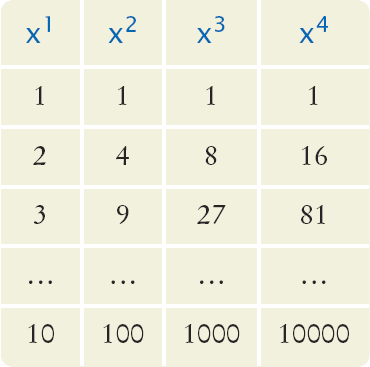
\includegraphics[height=0.5\paperheight,center]{pucrs-ep-fprog-unidade_04-lacos-laminas-tabela.png}
\end{figure}
	\end{column}
\end{columns}
\end{frame}

%-------------------------------------------------------
\begin{frame}\frametitle{Fluxograma de Dois Laços Aninhados}
\begin{figure}[h]
	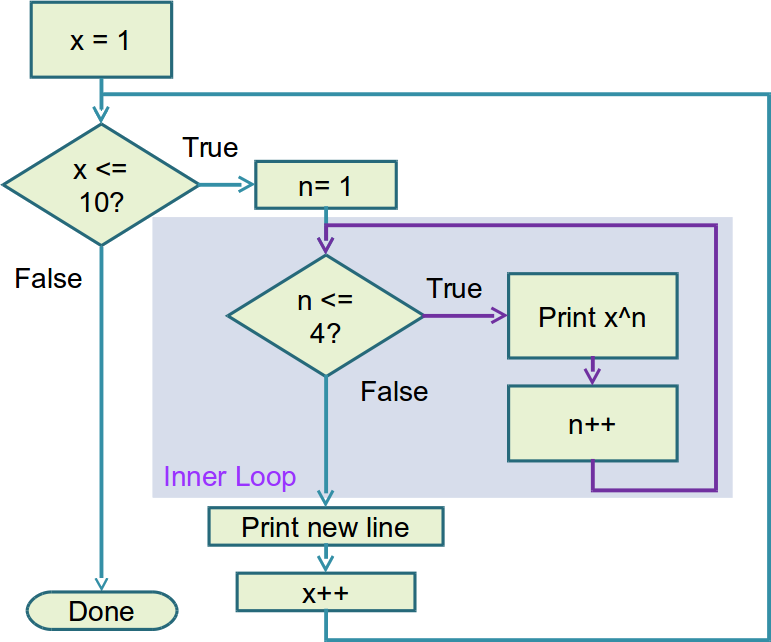
\includegraphics[height=0.65\paperheight,center]{pucrs-ep-fprog-unidade_04-lacos-laminas-fluxograma_lacos_aninhados.png}
\end{figure}
\end{frame}

%-------------------------------------------------------
\begin{frame}[fragile]\frametitle{\texttt{PowerTable.java} {\tiny (HORSTMANN, 2013, p. 173-174)}}
{\tiny
\begin{javacode}
/** This program prints a table of powers of x. */
public class PowerTable {
   public static void main(String[] args) {
      final int NMAX = 4;
      final double XMAX = 10;

      // Print table header
      for (int n = 1; n <= NMAX; n++) {
         System.out.printf("%10d", n);
      }
      System.out.println();
      for (int n = 1; n <= NMAX; n++) {
         System.out.printf("%10s", "x ");
      }
      System.out.println();

      // Print table body
      for (double x = 1; x <= XMAX; x++) {
         // Print table row
         for (int n = 1; n <= NMAX; n++) {
            System.out.printf("%10.0f", Math.pow(x, n));
         }
         System.out.println();
      }
   }
}
\end{javacode}
}
\end{frame}

%-------------------------------------------------------
\begin{frame}\frametitle{Resultado de \texttt{PowerTable.java}}
\begin{figure}[h]
	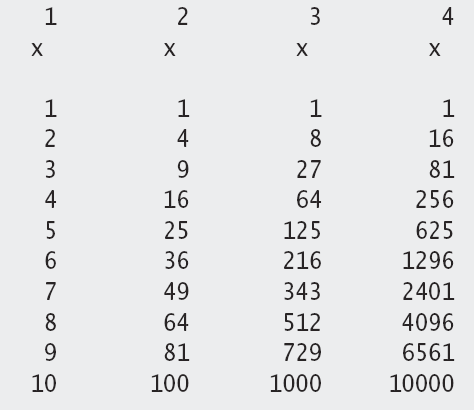
\includegraphics[height=0.65\paperheight,center]{pucrs-ep-fprog-unidade_04-lacos-laminas-resultado_de_powertable.png}
\end{figure}
\end{frame}

%-------------------------------------------------------
\begin{frame}[fragile]\frametitle{Exercício}
Modifique o programa \texttt{PowerTable.java} para que a tabela seja impressa ``deitada'', ou seja, na primeira linha os valores para $x^1$, na segunda linha os valores para $x^2$, e assim por diante.
\end{frame}

%-------------------------------------------------------
\begin{frame}[fragile]\frametitle{Exemplos de Laços Aninhados (1)}
\begin{center}
  \begin{tabular}{|p{6cm}|p{2cm}|p{5cm}|}
\hline
    \textbf{Laço} & \textbf{Saída} & \textbf{Explicação} \\
\hline
{\tiny
\begin{minted}{java}
for (i = 1; i <= 3 ; i++) {
   for (j = 1; j <= 4; j++) {
      System.out.print("*");
   }
   System.out.println();
}
\end{minted}
}
&
{\tiny
\begin{verbatim}
****
****
****
\end{verbatim}
}
& Imprime 3 linhas de 4 asteriscos cada.\\
\hline
{\tiny
\begin{minted}{java}
for (i = 1; i <= 4 ; i++) {
   for (j = 1; j <= 3; j++) {
      System.out.print("*");
   }
   System.out.println();
}
\end{minted}
}
&
{\tiny
\begin{verbatim}
***
***
***
***
\end{verbatim}
}
& Imprime 4 linhas de 3 asteriscos cada.\\
\hline
  \end{tabular}
\end{center}
\end{frame}

%-------------------------------------------------------
\begin{frame}[fragile]\frametitle{Exemplos de Laços Aninhados (2)}
\begin{center}
  \begin{tabular}{|p{6cm}|p{2cm}|p{5cm}|}
\hline
    \textbf{Laço} & \textbf{Saída} & \textbf{Explicação} \\
\hline
{\tiny
\begin{minted}{java}
for (i = 1; i <= 4 ; i++) {
   for (j = 1; j <= i; j++) {
      System.out.print("*");
   }
   System.out.println();
}
\end{minted}
}
&
{\tiny
\begin{verbatim}
*
**
***
****
\end{verbatim}
}
& Imprime 4 linhas com tamanhos 1, 2, 3 e 4.\\
\hline
{\tiny
\begin{minted}{java}
for (i = 1; i <= 3 ; i++) {
   for (j = 1; j <= 5; j++) {
      if (j % 2 == 0) {
         System.out.print("*");
      }
      else {
         System.out.print("-");
      }
   }
   System.out.println();
}
\end{minted}
}
&
{\tiny
\begin{verbatim}
-*-*-
-*-*-
-*-*-
\end{verbatim}
}
& Imprime asteriscos nas colunas pares e traços nas colunas ímpares.\\
\hline
  \end{tabular}
\end{center}
\end{frame}

%-------------------------------------------------------
\begin{frame}[fragile]\frametitle{Exemplos de Laços Aninhados (3)}
\begin{center}
  \begin{tabular}{|p{6cm}|p{2cm}|p{5cm}|}
\hline
    \textbf{Laço} & \textbf{Saída} & \textbf{Explicação} \\
\hline
{\tiny
\begin{minted}{java}
for (i = 1; i <= 3 ; i++) {
   for (j = 1; j <= 5; j++) {
      if (i % 2 == j % 2) {
         System.out.print("*");
      }
      else {
         System.out.print(" ");
      }
   }
   System.out.println();
}
\end{minted}
}
&
{\tiny
\begin{verbatim}
* * *
 * * 
* * *
\end{verbatim}
}
& Imprime o padrão de um tabuleiro de damas.\\
\hline
  \end{tabular}
\end{center}
\end{frame}

%-------------------------------------------------------
\begin{frame}[fragile]\frametitle{Exercício}
{\scriptsize
Faça laços aninhados para imprimir:
\begin{columns}[T]
	\begin{column}{0.34\linewidth}
\begin{enumerate}[a)]
	\item
\begin{verbatim}
*....
.*...
..*..
...*.
....*
\end{verbatim}
	\item
\begin{verbatim}
*****
.****
..***
...**
....*
\end{verbatim}
	\item
\begin{verbatim}
.....
*....
**...
***..
****.
\end{verbatim}
\end{enumerate}
	\end{column}
	\begin{column}{0.33\linewidth}
\begin{enumerate}[a)]
  \setcounter{enumi}{3}
	\item
\begin{verbatim}
....*
...*.
..*..
.*...
*....
\end{verbatim}
	\item
\begin{verbatim}
*****
****.
***..
**...
*....
\end{verbatim}
	\item
\begin{verbatim}
....*
...**
..***
.****
*****
\end{verbatim}
\end{enumerate}
	\end{column}
	\begin{column}{0.33\linewidth}
\begin{enumerate}[a)]
  \setcounter{enumi}{6}
	\item
\begin{verbatim}
*****
.***.
..*..
.....
.....
\end{verbatim}
	\item
\begin{verbatim}
*...*
.*.*.
..*..
.*.*.
*...*
\end{verbatim}
	\item
\begin{verbatim}
.....
.....
..*..
.***.
*****
\end{verbatim}
\end{enumerate}
	\end{column}
\end{columns}
}
\end{frame}

%=======================================================
\section{Resolução de Problemas: Storyboards (Esboços Sequenciais)}

%-------------------------------------------------------
\begin{frame}\frametitle{Resolução de Problemas: \emph{Storyboards} (Esboços Sequenciais)}
\begin{itemize}
	\item Um storyboard (esboço sequencial) consiste numa sequência de desenhos anotados para cada etapa de uma sequência de ações
	\item Trata-se de uma técnica útil para solução de problemas que permite modelar a interação com o usuário
	\item Pode ajudar a responder:
	\begin{itemize}
		\item Qual informação o usuário deve fornecer e em que ordem?
		\item Qual informação o programa deve mostrar e em que formato?
		\item O que deve acontecer se houver um erro?
		\item Quando o programa deve terminar?
	\end{itemize}
\end{itemize}
\end{frame}

%-------------------------------------------------------
\begin{frame}\frametitle{Exemplo de \emph{Storyboard}}
\begin{itemize}
	\item Objetivo: converter uma sequência de medidas
	\begin{itemize}
		\item Exigirá um laço e algumas variáveis
		\item Deverá gerenciar uma conversão de cada vez através de um laço
	\end{itemize}
\begin{figure}[h]
	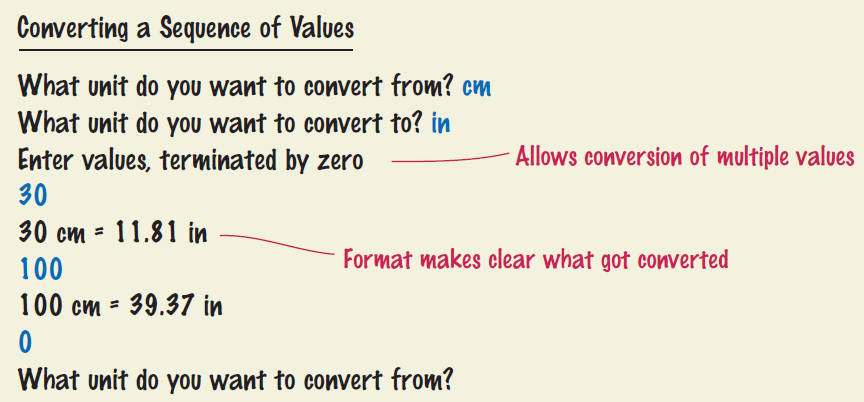
\includegraphics[height=0.5\paperheight,center]{pucrs-ep-fprog-unidade_04-lacos-laminas-storyboards1.jpg}
\end{figure}
\end{itemize}
\end{frame}

%-------------------------------------------------------
\begin{frame}\frametitle{O que pode dar errado?}
\begin{itemize}
	\item Unidades de medidas desconhecidas
	\begin{itemize}
		\item Como centímetros e polegadas são digitados?
		\item Que outras conversões estão disponíveis?
	\end{itemize}
	\item Solução: mostra uma lista de tipos de unidades aceitáveis
\begin{figure}[h]
	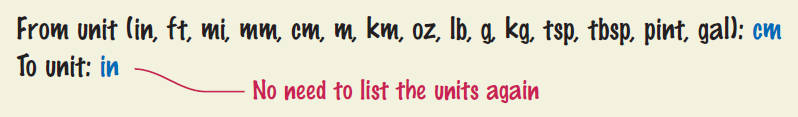
\includegraphics[height=0.15\paperheight,center]{pucrs-ep-fprog-unidade_04-lacos-laminas-storyboards2.jpg}
\end{figure}
\end{itemize}
\end{frame}

%-------------------------------------------------------
\begin{frame}\frametitle{O que mais pode dar errado?}
\begin{itemize}
	\item Como o usuário encerra o programa?
\begin{figure}[h]
	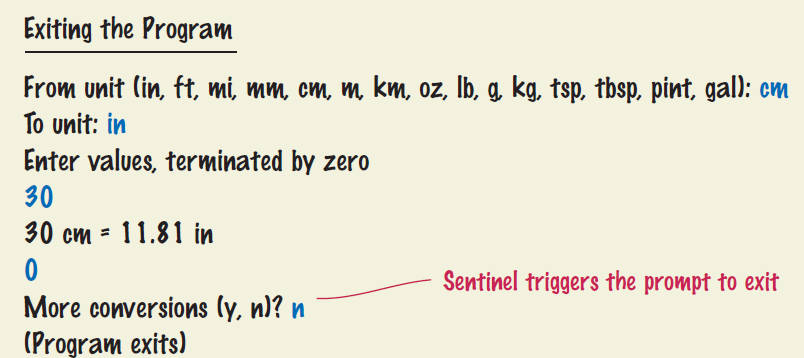
\includegraphics[height=0.5\paperheight,center]{pucrs-ep-fprog-unidade_04-lacos-laminas-storyboards3.jpg}
\end{figure}
	\item Storyboards ajudam a planejar um programa: conhecer os fluxos ajuda a estruturar o código
\end{itemize}
\end{frame}

%=======================================================
\section{Resumo}

%-------------------------------------------------------
\begin{frame}\frametitle{Resumo (1)}
\begin{itemize}
	\item Há 3 tipos de laços:
	\begin{itemize}
		\item Laços \texttt{while}
		\item Laços \texttt{for}
		\item Laços \texttt{do}
	\end{itemize}
	\item Cada laço possui as seguintes seções:
	\begin{itemize}
		\item Inicialização (preparação das variáveis para iniciar o laço)
		\item Condição (teste para verificar se o corpo do laço deve ser executado)
		\item Atualização (alteração de alguma variável testada na condição)
	\end{itemize}
\end{itemize}
\end{frame}

%-------------------------------------------------------
\begin{frame}\frametitle{Resumo (2)}
\begin{itemize}
	\item Um laço executa instruções repetidamente enquanto uma condição for verdadeira
	\item Errar o número de iterações em laço por uma unidade é um erro comum de programação
	\begin{itemize}
		\item Procure deixar os testes simples para evitar este tipo de erro.
	\end{itemize}
	\item O laço \texttt{for} é usado quando um valor varia de um ponto de partida até um ponto final com um incremento ou decremento constante
	\item O laço \texttt{do} é apropriado quando o corpo do laço deve ser executado pelo menos uma vez
\end{itemize}
\end{frame}

%-------------------------------------------------------
\begin{frame}\frametitle{Resumo (3)}
\begin{itemize}
	\item Um valor de sentinela consiste de um valor que determina o final de um conjunto de dados, mas que não faz parte deste conjunto
	\item Você pode usar uma variável booleana para controlar um laço
	\begin{itemize}
		\item Defina a variável com \texttt{true} antes de entrar no laço, e então defina ela com \texttt{false} para sair do laço
	\end{itemize}
	\item Quando o corpo de um laço contiver outro laço, os laços são aninhados
	\begin{itemize}
		\item Um uso típico para laços aninhados é a impressão de uma tabela com linhas e colunas
	\end{itemize}
	\item Em uma simulação, o computador é usado para simular uma atividade
	\begin{itemize}
		\item Pode-se introduzir aleatoriedade chamando o gerador de números aleatórios
	\end{itemize}
\end{itemize}
\end{frame}

%=======================================================
\section{Tópicos Avançados}

%-------------------------------------------------------
\begin{frame}[fragile]\frametitle{Tópicos Avançados}
\begin{itemize}
	\item Números Aleatórios e Simulações
\end{itemize}
\end{frame}

%-------------------------------------------------------
\begin{frame}\frametitle{Números Aleatórios e Simulações}
\begin{itemize}
	\item Jogos frequentemente usam números aleatórios para tornar as coisas mais interessantes
	\begin{itemize}
		\item Jogar dados
		\item Girar uma roda
		\item ``Comprar'' uma carta
	\end{itemize}
	\item Uma simulação usualmente envolve executar um laço para uma sequência de eventos
	\begin{itemize}
		\item Dias
		\item Eventos
	\end{itemize}
\end{itemize}
\end{frame}

%-------------------------------------------------------
\begin{frame}[fragile]\frametitle{Exemplo: \texttt{RandomDemo.java} {\tiny [Publicado em Horstmann (2013, p. 176)]}}
\begin{itemize}
	\item O método \texttt{Math.random()} pode ser usado para gerar números aleatórios no intervalo [0;1)
\end{itemize}
\scriptsize{\inputminted[bgcolor=cyan!10]{java}{src/RandomDemo.java}}
\end{frame}

%-------------------------------------------------------	
\begin{frame}[fragile]\frametitle{Resultado de \texttt{RandomDemo.java}}
\begin{javacode}
0.6513550469421886
0.920193662882893
0.6904776061289993
0.8862828776788884
0.7730177555323139
0.3020238718668635
0.0028504531690907164
0.9099983981705169
0.1151636530517488
0.1592258808929058
\end{javacode}
\end{frame}

%-------------------------------------------------------
\begin{frame}[fragile]\frametitle{Simulando o Lançamento de Dados}
\begin{columns}[T]
	\begin{column}{0.7\linewidth}
\begin{itemize}
	\item Objetivo: obter valores inteiros aleatórios entre 1 e 6
	\item \texttt{Dice.java} (HORSTMANN, 2013, p. 177)
{\scriptsize
\begin{javacode}
/** This program simulates tosses of a pair of dice. */
public class Dice {
   public static void main(String[] args) {
      for (int i = 1; i <= 10; i++) {
         // Generate two random numbers between 1 and 6
         int d1 = (int) (Math.random() * 6) + 1;
         int d2 = (int) (Math.random() * 6) + 1;
         System.out.println(d1 + " " + d2);
      }
   }
}
\end{javacode}
}
\end{itemize}
	\end{column}
	\begin{column}{0.3\linewidth}
\begin{itemize}
	\item Resultado de \texttt{Dice.java}:
{\scriptsize
\begin{javacode}
5 1
2 1
1 2
5 1
1 2
6 4
4 4
6 1
6 3
5 2
\end{javacode}
}
\end{itemize}
	\end{column}
\end{columns}
\end{frame}

%-------------------------------------------------------
\begin{frame}\frametitle{O Método Monte Carlo}
\begin{itemize}
	\item Usado para encontrar soluções aproximadas para problemas que não podem ser resolvidos com precisão
	\item Exemplo: aproximar o valor de PI usando áreas relativas de um círculo dentro de um quadrado
	\begin{itemize}
		\item Usa aritmética simples
		\item Hits (Acertos) estão dentro do círculo
		\item Tries são o número total de tentativas
		\item Razão é 4 x Hits / Tries
	\end{itemize}
\begin{figure}[h]
	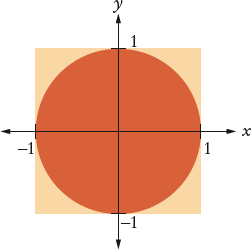
\includegraphics[height=0.2\paperheight,center]{pucrs-ep-fprog-unidade_04-lacos-laminas-monte_carlo.png}
\end{figure}
\end{itemize}
\end{frame}

%-------------------------------------------------------
\begin{frame}[fragile]\frametitle{\texttt{MonteCarlo.java} {\tiny (HORSTMANN, 2013, p. 178-179)}}
{\tiny
\begin{javacode}
/**
   This program computes an estimate of pi by simulating dart throws onto a square.
*/
public class MonteCarlo {
   public static void main(String[] args) {
      final int TRIES = 10000;
      int hits = 0;
      for (int i = 1; i <= TRIES; i++) {
         // Generate two random numbers between -1 and 1
         double r = Math.random();
         double x = -1 + 2 * r; // Between -1 and 1
         r = Math.random();
         double y = -1 + 2 * r;
         // Check whether the point lies in the unit circle
         if (x * x + y * y <= 1) { hits++; }
      }
      /* The ratio hits / tries is approximately the same as the ratio
         circle area / square area = pi / 4  */
      double piEstimate = 4.0 * hits / TRIES;
      System.out.println("Estimate for pi: " + piEstimate);
   }
}
\end{javacode}
~\\
~\\
Resultado:\\
\begin{javacode}
Estimate for pi: 3.1504
\end{javacode}
}
\end{frame}

%=======================================================
\section{Referências}

%-------------------------------------------------------
\begin{frame}\frametitle{Referências}
\noindent{HORSTMANN, C. \textbf{Java for Everyone – Late Objetct}. 2. ed. Hoboken: Wiley, 2013. xxxiv, 589 p.}
\end{frame}

%=======================================================
\end{document}

